%!TEX root = ../Report.tex
\chapter{Analysis of Data}
\label{chp:analysis}

This chapter provides some examples of tables and graphs. Examples are from the \acf{CUMACF} methodology.

\section{Usage Adherence Data}

Table~\ref{tab:usage} shows a fictive data set for usage adherence. All number are days. 
%
Using the following simple formula, adherence pr.\ participant can be calculated, as shown in the last column of Table~\ref{tab:usage}:

\[
    adherence = \frac{usage}{length-downtime}
\]

Note that the \emph{instructed} number of days are not included in the calculation of adherence. However, if the actual length of study for each participant is unavailable, the instructed length may substitute this. This will, off course, provide a lower adherence rate.
Note also, that the \textit{total adherence} is calculated using the formula above -- in this case it is 92\%. 
Using the average of each participant's adherence rate is, however, misleading as the overall adherence rate. This is illustrated in Table~\ref{tab:usage}, where the average adherence rate is 87\%. This is lower, since the adherence rate for the `short' studies (P7 and P8) are low.


\begin{table}[htp]
\caption{Example of usage adherence data collected. In this example, all reported number are days of a study.}
\centering
\scriptsize
\begin{tabular}{|c|c|c|c|c|c|}
\hline
\textbf{participant}	& \textbf{instr.} &	\textbf{lenght} &	\textbf{downtime} &	\textbf{usage} &	\textbf{adherence} \\
\hline
\hline
P1 &	183	&   170 &	3 &	165 &	99\%\\
P2 &	183 &	120 &	2 & 101 &	86\%\\
P3 &	183 &	73  &	2 &	45  &	63\%\\
P4 &	183 &	173	&   1 &	156 &	91\%\\
P5 &	183 &	108	&   1 &	105	&   98\%\\
P6 &	122 &	93	&   1 &	91	&   99\%\\
P7 &	61  &	45	&   2 &	23	&   53\%\\
P8 &	30  &	23	&   0 &	20	&   87\%\\
P9 &	183 &	194	&   1 &	191	&   99\%\\
P10 &	183 &	118	&   3 &	115	&   100\%\\
\hline
\textbf{total} & &		1.117 &	16 &	1.012 & 	\textbf{92\%}\\
\hline
\textbf{avg.} & & & & &					\textbf{87\%}\\
\hline
\hline
\end{tabular}
\label{tab:usage}
\end{table}


\begin{figure}[!ht]
    \centering
    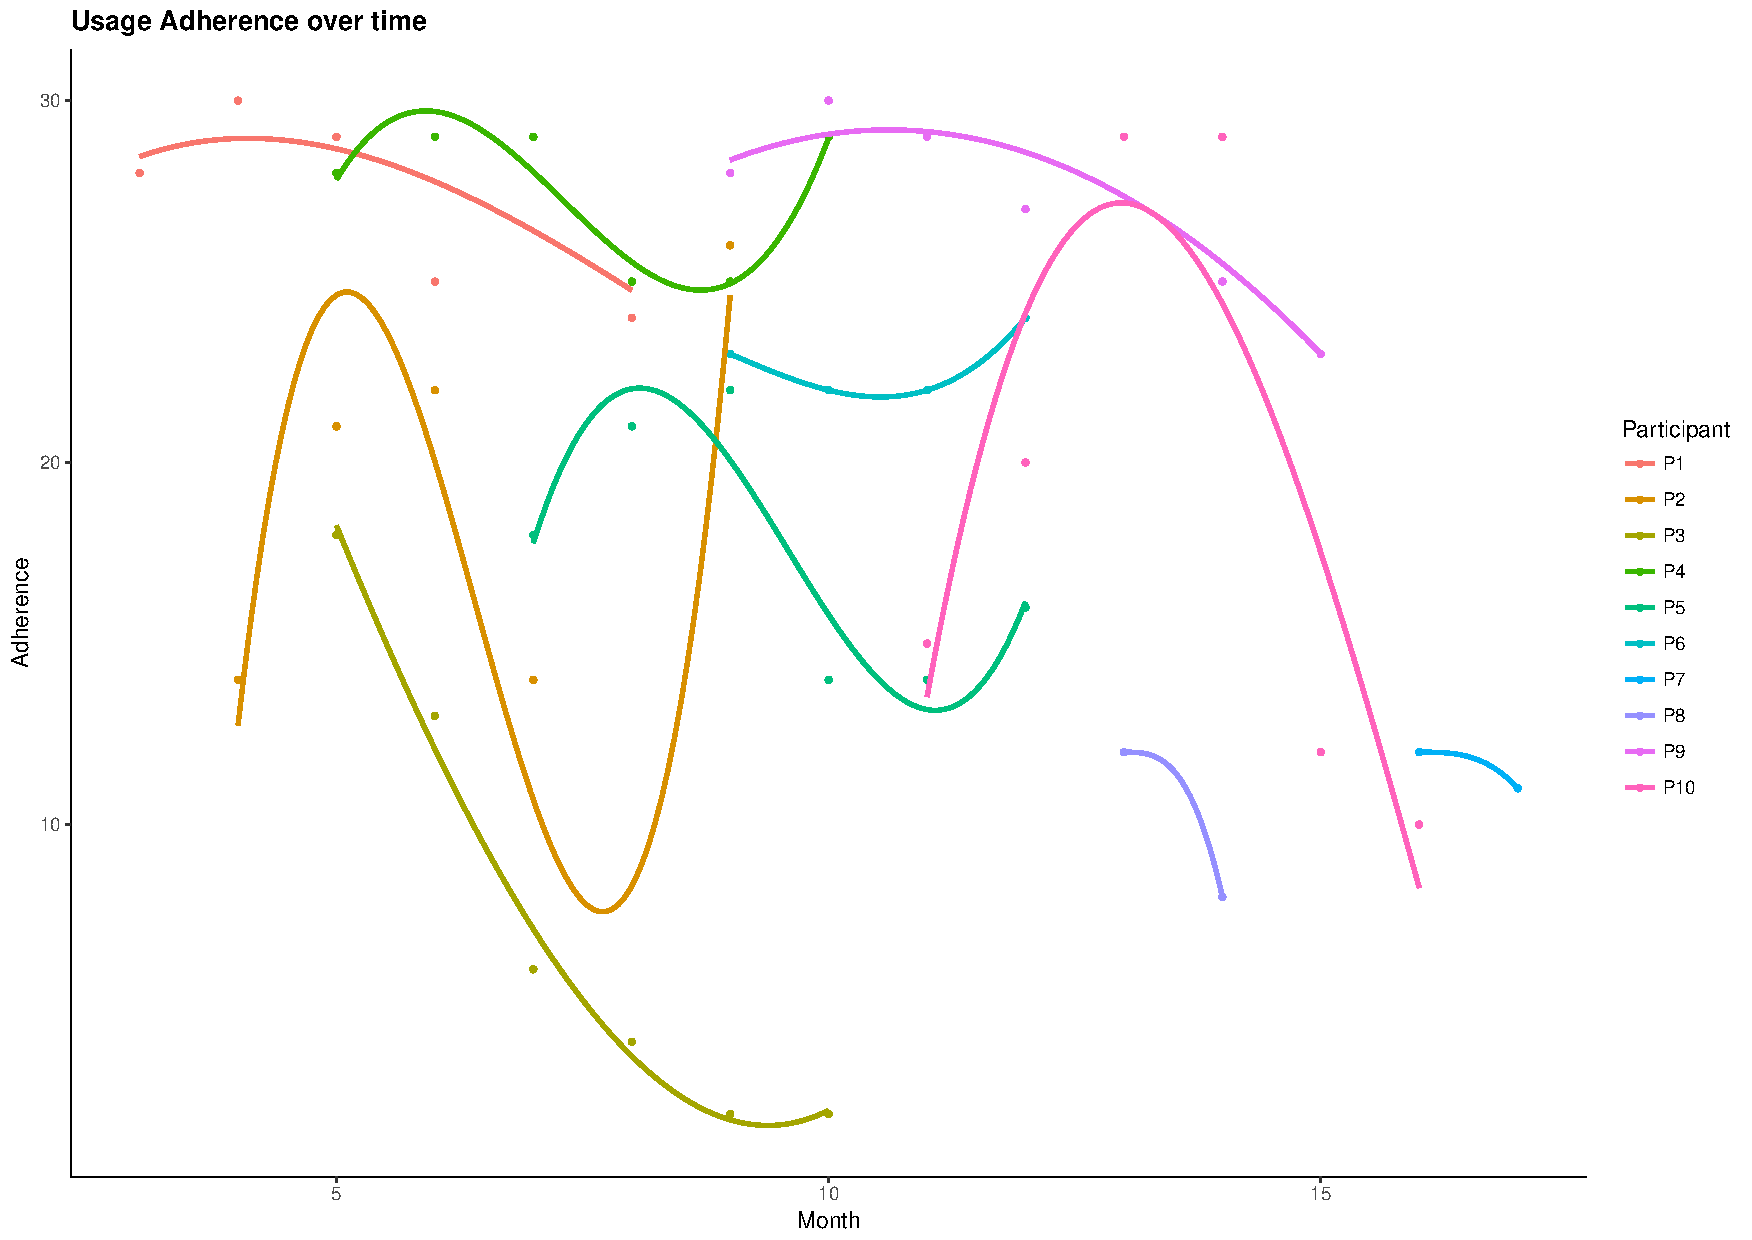
\includegraphics[width=0.7\textwidth]{./images/adherence_R_plot.pdf}
    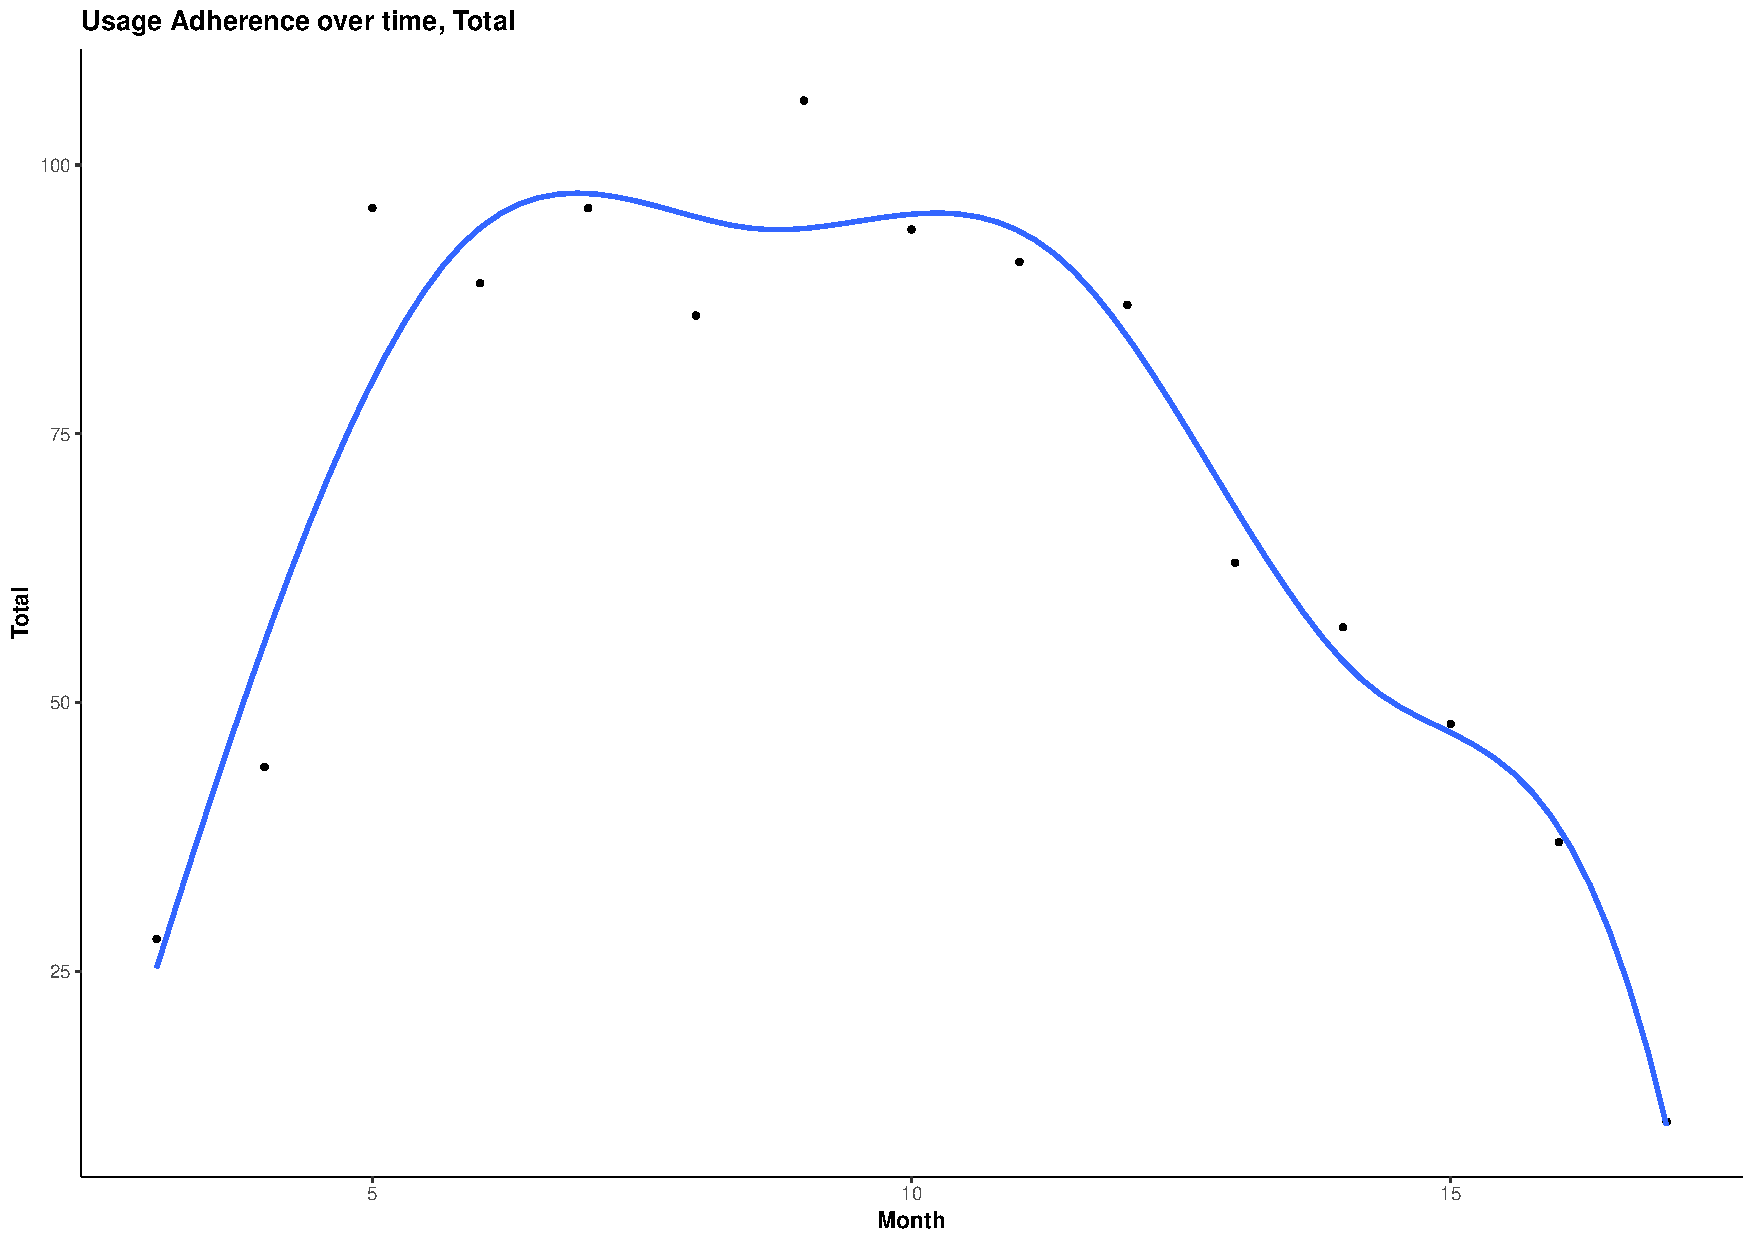
\includegraphics[width=0.7\textwidth]{./images/adherence_total_R_plot.pdf}
    \caption{Usage of a system over time. Top: Usage patterns for each of the ten participants. Bottom: Total usage pattern}
    \label{fig:usage}
\end{figure}


Figure~\ref{fig:usage} provides an example of how to illustrate usage adherence over time. In this example, the usage from the ten participants listed in Table~\ref{tab:usage} is shown on a monthly basis over a period of 15 month (month 3 to 17). 
%
The top figure shows the usage patterns for each of the ten participants with a smoothed curve fitted to the data points. 
Participants show different usage patterns. For example, P2 initially starts using the system, but ends up with limited use of the system, whereas P10 starts out low, but gradually increase her/his usage.
The bottom figure shows the overall usage. This latter figure can illustrate the overall diffusion of the technology. According to the theory of diffusion of technology (innovation), this should be a normal distribution over time~\cite{rogers2003diffusion}. This trend is recognized in Figure~\ref{fig:usage}; usage gradually grows from month 3, raising to a plateau in months 7 to 12, after which it declines. This patterns is, of course, contingent to the specific details of the study; in our example, the study period is 6 months and participants did not use the system beyond this period.
%
Figure~\ref{fig:usage} is generated from an R script, which is available in Appendix~\ref{app:r_script}.


\section{Perceived Usefulness and Usability Data}

The \ac{CUMACF} questionnaire is applying a 5-point Likert scale of; `strongly disagree', `disagree', `neither agree nor disagree', `agree', and `strongly agree', with numerical scores from 1--5.
%
The question is how to represent the results of a survey using such a 5-point Likert. 
%
One common practice is to take the mean. However, as pointed out by Robbins et al.~\cite{robbins2011plotting}, it is controversial since there is no assurance that there is even spacing between the descriptions of attitude. There is no reason to assume that the distance between agree and strongly agree is the same as the distance from agree to neither agree nor disagree. However, even if it were acceptable to take means, it is not very useful. 
%
For example, if we look at the example survey data in Table~\ref{tab:survey}, the first three questions (HE1--3) provides the same mean ($24.0$), but there is a big difference between HE1 where respondents are concentrated at both ends of the scale, and HE2 in which all respondents are all neutral. Hence, based on the response to HE1 it would be very wrong to conclude that ``on average, respondents were \textit{neutral} as to whether the system would be useful for handling diabetes''.


\begin{table}[htp]
\caption{Example of survey data from the \ac{CUMACF} perceived usefulness and usability questionnaire. The center figures are the number of respondents in each category, and total and average scores are on the right.}
\centering
\scriptsize
\begin{tabular}{|c p{2.0cm}| c c c c c | c c|}
\toprule 
\hline
\textbf{}	& \textbf{} &	\textbf{Strongly} &	\textbf{} &	\textbf{} &	\textbf{}  &	\textbf{Strongly}  &	\multicolumn{2}{c|}{\textbf{Scores}} \\
\textbf{\#}	& \textbf{Question} &	\textbf{Disagree} &	\textbf{Disagree} &	\textbf{Neutral} &	\textbf{Agree}  &	\textbf{Agree}  &	\textbf{Total}  &	\textbf{Avg.} \\
\hline
\hline
HE1	& Usefulness    &	20 & 	 0 & 	 0 & 	 0 & 	20 & 	120 &	24.0\\
HE2	& Adherence     &	 0 & 	 0 & 	40 & 	 0 & 	 0 & 	120 &	24.0\\
HE3	&Behavior       &	10 & 	10 & 	 0 & 	10 & 	10 & 	120 &	24.0\\
HE4	& Health        &	12 & 	 2 & 	 4 & 	 6 &	23 & 	167 &	33.4\\
HE5	& Efficiency    &	 2 & 	14 &	32 & 	21 & 	 3 &	225 &	45,0\\
HE6	& Productivity  &	32 & 	 2 & 	 3 &	12 & 	 2 & 	103 &   20.6\\
HE7	& Quality       &	10 & 	 2 & 	 4 &	 1 & 	23 &	145 &	29.0\\
HE8	& Safety        &	 4 &	14 &     2 & 	33 & 	 3 & 	185 &   37.0\\
\hline
EE1	& Usability     &	12 & 	 2 & 	 5 &	 2 & 	 3 &	 54 &	10.8\\
EE2	& Understandable &	10 & 	 2 & 	 4 & 	 6 &	23 & 	165 &	33.0\\
EE3	& Learning      &	 4 &	 2 & 	23 &    12 & 	11 & 	180 &	36.0\\
EE4	& Easy          &	28 &	11 & 	 5 &	 4 &	 3 &	 96 &	19.2\\
EE5	& Skillful      &	18 &	 2 & 	 4 &	 6 &	11 & 	113 &	22.6\\
EE6	& Information   &    4 &	14 &    32 & 	15 &	 3 &	203 &   40.6\\
EE7	& Interface     &	 5 &	21 & 	 5 &	 4 &	 3 &	 92 &	18.6\\
EE8	& Pleasure      &	12 &	14 &	11 &	 3 &	 4 &	105 &	21.0\\
EE9	& Features      & 	 4 &	 4 &     3 &	44 &	12 &	257 &   51.4\\
\hline
\bottomrule
\end{tabular}
\label{tab:survey}
\end{table}

Robbins et al.~\cite{robbins2011plotting} discuss different ways to present and visualize Likert scale data and recommend to present data in (i) a table and (ii) as a so-called `diverging stacked bar chart' As an example, we can look at the data in Table~\ref{tab:survey}, which is visualized in a diverging stacked bar chart in Figure~\ref{fig:chart}.
Figure~\ref{fig:chart} is generated from an R script (originally proposed by Heiberger \& Robbins~\cite{heiberger2014design}). The R script is available in Appendix~\ref{app:r_script}.



% \begin{figure}[!ht]
%     \centering
%     \includegraphics[width=1.0\textwidth]{./images/survey.pdf}
%     \caption{Percentages for Agreement that primary position is professionally challenging by demographics characteristics~\cite{robbins2011plotting}}
%     \label{fig:survey}
% \end{figure}


\begin{figure}[!ht]
    \centering
    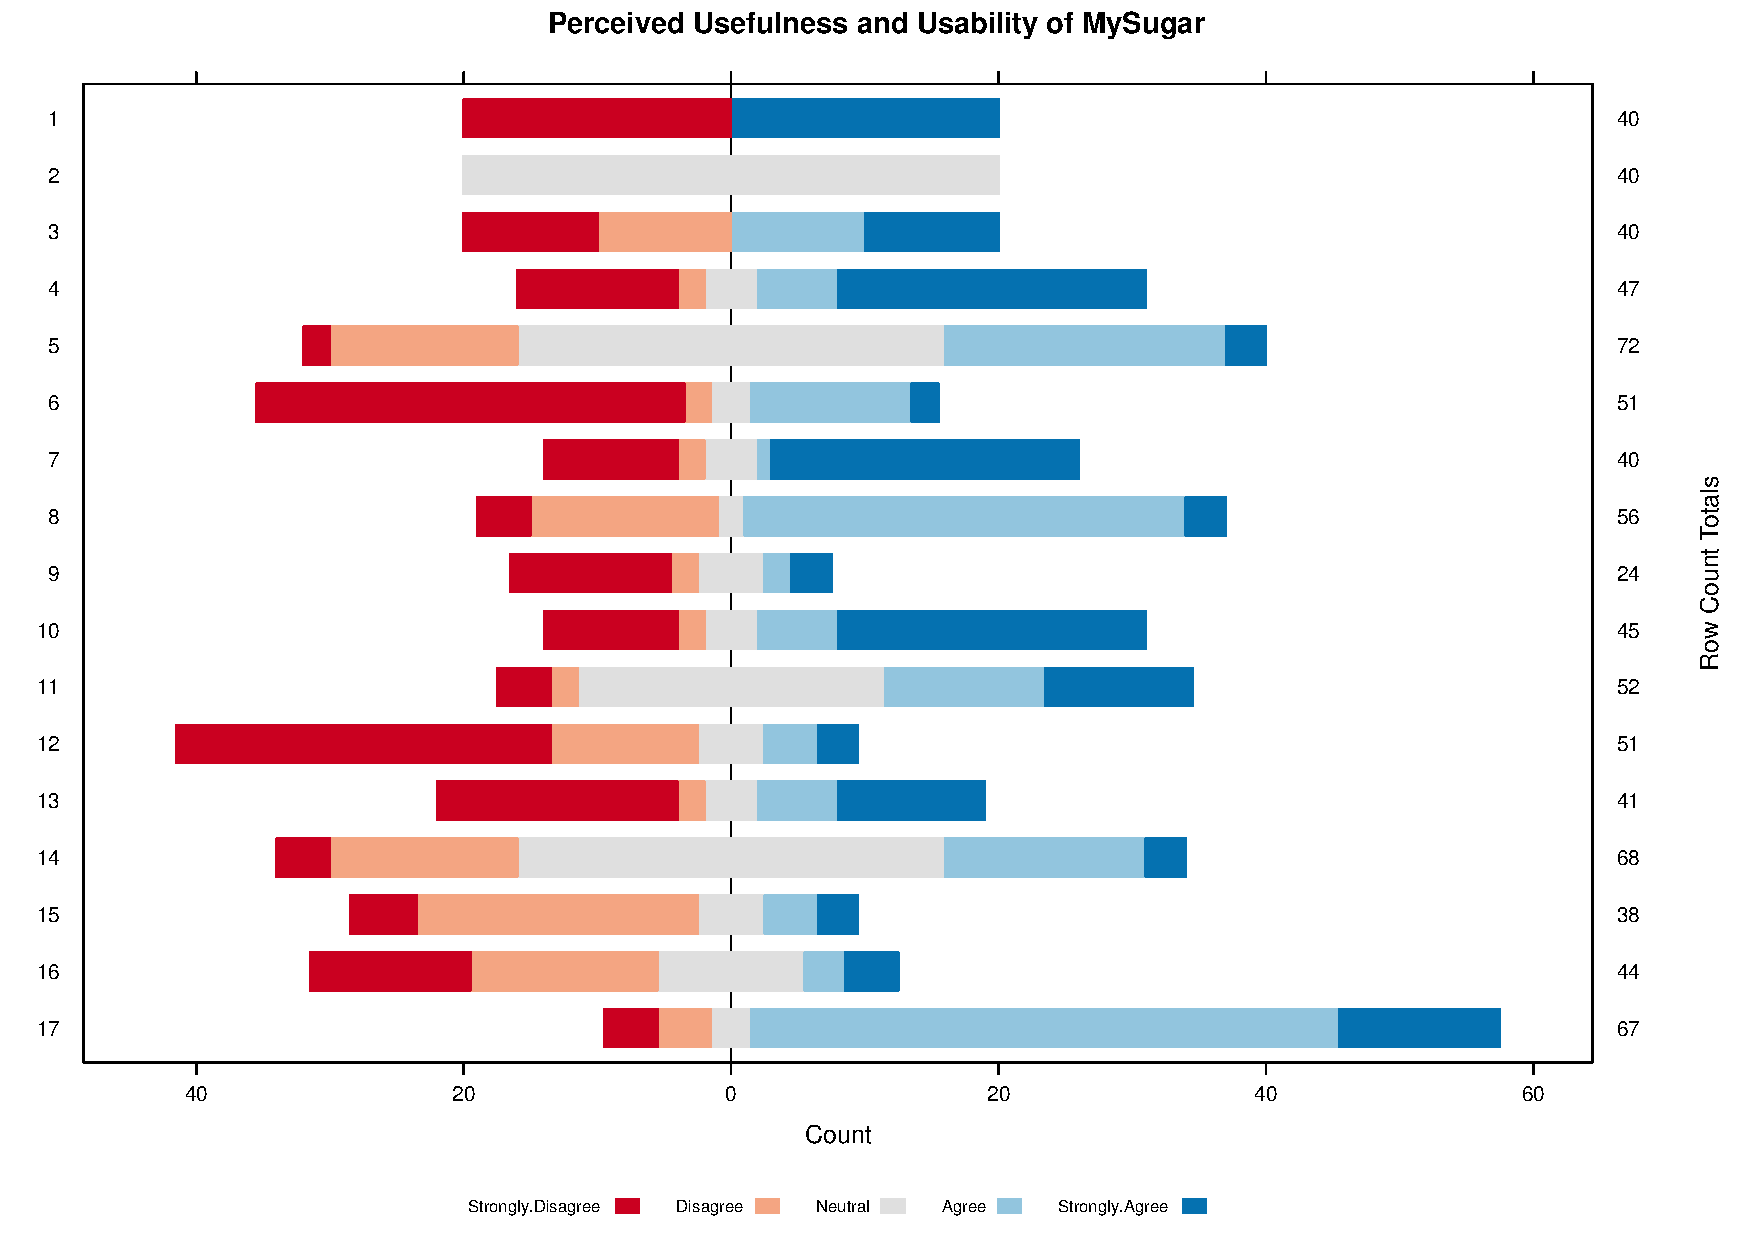
\includegraphics[width=1.0\textwidth]{./images/survey_R_plot.pdf}
    \caption{Diverging stacked bar chart of the data in Table~\ref{tab:survey}}
    \label{fig:chart}
\end{figure}
